\section{Theoretical Analysis}
\label{sec:analysis}
\paragraph{}
\par In this section, the circuit shown in Figure \ref{circuit} is analysed
theoretically, using the two methods required, mesh and nodes. The known values can be checked in the table below.
\begin{table}[H]
    \centering
    \begin{tabular}{|c|c|}
    \hline
        $R_1$ & 1.01080769792 kOhm \\ \hline 
        $R_2$ & 2.07664633274 kOhm \\ \hline
        $R_3$ & 3.12595649013 kOhm \\ \hline
        $R_4$ & 4.18722214507 kOhm \\ \hline
        $R_5$ & 3.0841699201 kOhm  \\ \hline
        $R_6$ & 2.00179338129 kOhm \\ \hline
        $R_7$ & 1.04556537884 kOhm \\ \hline
        $V_a$ & 5.00120775651 V \\ \hline
        $I_d$ & 1.03136220214 mA \\ \hline
        $K_b$ & 7.12593545434 mS \\ \hline
        $K_c$ & 8.24048597287 kOhm \\ \hline	
    \end{tabular}
    \caption{Known Data}
    \label{data}
\end{table}
\subsection{Mesh Method}
\paragraph{}
\par A mesh is a loop that contains no other loops within it. That said, the mesh method is able to determine the current in each of the said loops, resorting to the Kirchoff Voltage Law (KVL). Having those values it is a matter of applying Ohms Law to the resistances in the mesh in order to determine the voltage in every node in the circuit, given that the values for the resistances are provided. This method is not common in automation because it is necessary to identify the different meshes, to which there may be a necessity for an outside observer.

\par Analyzing our circuit in particular, we can identify four meshes, to which we wrote the equations, stipulating a current flow for each mesh, as shown in figure \ref{mesh}. 

\begin{figure}[H]
    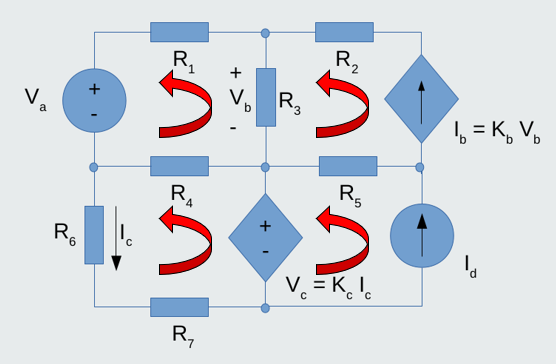
\includegraphics[width=0.5\linewidth]{Mesh.png}
    \centering
    \caption{Mesh Method applied to the circuit}
    \label{mesh}
\end{figure}

\par After simplyfying the mesh method, the system \ref{system mesh} was obtained as follows
$$
\begin{cases} 
	R_{1}I_{a}+R_{3}(I_{a}-I_{b})+R_{4}(I_{a}-I_{c}) = V_a \\ 
	R_{3}(I_{a}-I_{b})+\frac{I_{b}}{K_{b}} = 0 \\
	R_{4}(I_{a}-I_{c})-R_{6}I_{c}-R_{7}I_{c}+K_{c}I_{c} = 0 
\label{system mesh}
\end{cases}
$$


\par It was then morphed into the system below \ref{matrix} and solved with the aid of \textit{Octave}. 

\begin{equation}
	\begin{bmatrix}
		R_1+R_3+R_4 & -R_3 & -R_4 \\
		R_3 & -R_3+\frac{1}{K_b} & 0 \\
		R_4 & 0 & K_c-R_4-R_6-R_7 \\
	\end{bmatrix}
	\begin{bmatrix}
		I_a     \\
		I_b     \\
		I_c \\
	\end{bmatrix}
    =
	\begin{bmatrix}
		V_a     \\
		0     \\
		0  \\
	\end{bmatrix}
	\label{matrix}
\end{equation}

\par It was possible, after the said, to obtain the values for the voltage and current sources, as can be verified in the following table \ref{mesh}, with the current measured in mA and the voltage in V. 

\begin{table}[H]
  \centering
  \begin{tabular}{|c|c|}
    \hline    
    {\bf Name} & {\bf Value [mA]} \\ \hline
    $I_a$ & 2.224637e-01 \\ \hline 
$I_b$ & 2.329201e-01 \\ \hline 
$I_c$ & -9.260366e-01 \\ \hline 
$I_d$ & 1.031362e+00 \\ \hline 

  \end{tabular}
  \caption{Mesh method results.}
  \label{mesh}
\end{table}
\newpage
\subsection{Node Method}
\paragraph{}
\par The most crucial part in this method is to properly identify all the nodes in a circuit, which are the regions that connect two or more elements of a circuit. Then, with the aid of a system of equations provided by the Kirchoff Current Law (KCL) in the nodes unrelated to voltage sources and some extra equalities, it is possible to determine the voltage in every node. Due to the fact that we can only use KCL like previously explained, the aforementioned extra equalities must be create some sort of connection between the nodes not analyzed and the current sources. Contrary to the Mesh method, it is simple to automate, given its straightforward approach, making it achievable to obtain values in a simulation.


\par Firstly, all the nodes were numbered and represented as shown in figure \ref{circuitlt}.
 
\begin{figure}[H]
    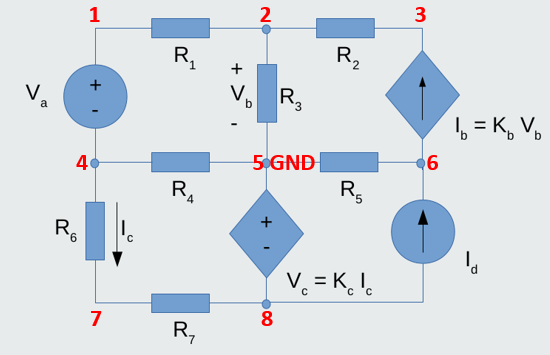
\includegraphics[width=0.8\linewidth]{Nodes.png}
    \centering
    \caption{Nodes Method applied to the circuit}
    \label{circuitlt}
\end{figure}


\par Then, the system of equations was written using the numeration stipulated above. There was a voltage source $V_T$ created to aid the analysis of the simulation.
$$
\begin{cases} 
	G_1(V_1-V_2)+G_2(V_3-V_2)-G_3V_b = 0 \\
	G_2(V_2-V_3)+V_b = 0 \\ 
	G_5(V_5-V_6)-V_b = -I_d \\
	G_6(V_4-V_7)-\frac{V_c}{K_c} = 0 \\
	G_7/(V_8-V_7)+\frac{V_c}{K_c} = 0 \\
	V_1-V_4 = V_a \\
	V_2-V_5-V_b = 0 \\
	V_5 = 0 \\
	V_5-V_8-V_c = 0 \\
	G_1(V_2-V_1)+G_4(V_5-V_4)-\frac{V_c}{K_c} = 0 
\label{system nodes}
\end{cases}
$$
\par The system above was then converted into a matrix equation \ref{matrixn} in order to have it solved by \textit{Octave}.
\begin{equation}
	\begin{bmatrix}
		G_1 & -G_1-G_2 & 0 & 0 & 0 & 0 & 0 & 0 & -G_3 & 0\\
		0 & G_2 & -G_2 & 0 & 0 & 0 & 0 & 0 & K_b & 0\\
		0 & 0 & 0 & 0 & G_5 & -G5 & 0 & 0 & -K_b & 0 \\
		0 & 0 & 0 & G_6 & 0 & 0 & -G_6 & 0 & 0 & -\frac{1}{K_c} \\
		0 & 0 & 0 & 0 & 0 & 0 & -G_7 & G_7 & 0 & \frac{1}{K_c} \\
		1 & 0 & 0 & -1 & 0 & 0 & 0 & 0 & 0 & 0\\
		0 & 1 & 0 & 0 & -1 & 0 & 0 & 0 & -1 & 0\\
		0 & 0 & 0 & 0 & 1 & 0 & 0 & 0 & 0 & 0\\
		0 & 0 & 0 & 0 & 1 & 0 & 0 & -1 & 0 & -1\\
		-G_1 & G_1 & 0 & -G_4 & G_4 & 0 & 0 & 0 & 0 & -\frac{1}{K_c} \\
	\end{bmatrix}
	\begin{bmatrix}
		V_1     \\
		V_2     \\
		V_3  \\
		V_4  \\
		V_5  \\
		V_6   \\
		V_7   \\ 
		V_8     \\
		V_b     \\
		V_c       \\
	\end{bmatrix}
    =
	\begin{bmatrix}
		0     \\
		0     \\
		-I_d  \\
		0     \\
		0     \\
		V_a     \\
		0     \\
		0     \\
		0     \\
		0     \\
	\end{bmatrix}
	\label{matrixn}
\end{equation}

\par With that, the values for $V_1$ up to $V_8$, $V_b$ and $V_c$ were achieved with the values afterwards displayed. The units for current and voltage are the same as in the mesh method.

\begin{table}[H]
  \centering
  \begin{tabular}{|c|c|}
    \hline    
    {\bf Name} & {\bf Value [V]} \\ \hline
    $V_5$ & 0.000000e+00 \\ \hline 
$V_1$ & 1.921818e-01 \\ \hline 
$V_2$ & -3.268625e-02 \\ \hline 
$V_3$ & -5.163789e-01 \\ \hline 
$V_4$ & -4.809026e+00 \\ \hline 
$V_6$ & 3.899261e+00 \\ \hline 
$V_7$ & -6.662760e+00 \\ \hline 
$V_8$ & -7.630992e+00 \\ \hline 
$V_a$ & 5.001208e+00 \\ \hline 
$V_b$ & -3.268625e-02 \\ \hline 
$V_c$ & 7.630992e+00 \\ \hline 

  \end{tabular}
  \caption{Nodes method results.}
  \label{tab:op}
\end{table}

\par It is now possible, with
\begin{equation}
	V_b=\frac{I_b}{K_b}
\label{Vb}
\end{equation}
and
\begin{equation}
	V_c=K_{c}I_{c}
\end{equation}
to obtain the values for all the voltages named in the circuit, $V_a$, $V_b$ and $V_c$:


\par It is visible that the values obtain in both methods present virtually identical values.

\par In the next section, these methods will be compared with a simulation of the circuit, with the aim of testing this theoretical analysis and discussing its results.
\newpage
